\documentclass[11pt,a4paper]{article}

% --- Essential Packages ---
\usepackage[utf8]{inputenc}
\usepackage[margin=0.85in]{geometry}
\usepackage{amsmath,amssymb}
\usepackage{xcolor}
\usepackage{tikz}
\usetikzlibrary{shapes,arrows.meta,positioning,calc,fit,backgrounds,decorations.pathreplacing}
\usepackage{tcolorbox}
\tcbuselibrary{skins,breakable}
\usepackage{booktabs}
\usepackage{enumitem}
\usepackage{listings}
\usepackage{hyperref}
\usepackage{fancyhdr}
\usepackage{titlesec}
\usepackage{microtype}

% --- Color Palette (Modern, Professional, Clean) ---
\definecolor{primaryblue}{RGB}{16, 76, 140}
\definecolor{secondaryblue}{RGB}{41, 128, 185}
\definecolor{accentteal}{RGB}{0, 150, 136}
\definecolor{darkslate}{RGB}{44, 62, 80}
\definecolor{lightbg}{RGB}{248, 249, 250}
\definecolor{alertred}{RGB}{192, 57, 43}
\definecolor{boxgold}{RGB}{212, 143, 24}

% --- Typography and Section Styles ---
\titleformat{\section}{\Large\bfseries\color{primaryblue}}{\thesection}{1em}{}[\titlerule]
\titleformat{\subsection}{\large\bfseries\color{secondaryblue}}{\thesubsection}{1em}{}
\titleformat{\subsubsection}{\normalsize\bfseries\color{darkslate}}{\thesubsubsection}{1em}{}

% --- Header and Footer ---
\pagestyle{fancy}
\fancyhf{}
\rhead{\color{gray}\small NanoSat TDOA: Master Field \& Theory Guide}
\lhead{\color{primaryblue}\bfseries Project NanoSat}
\rfoot{\color{gray}\small Page \thepage}
\renewcommand{\headrulewidth}{0.5pt}
\renewcommand{\footrulewidth}{0.5pt}

% --- Custom Callout Boxes ---
\newtcolorbox{conceptbox}[1]{
    colback=lightbg,
    colframe=secondaryblue,
    fonttitle=\bfseries\color{white},
    title=#1,
    sharp corners=south,
    rounded corners=north,
    boxrule=1.5pt,
    breakable
}

\newtcolorbox{safetybox}[1]{
    colback=red!5!white,
    colframe=alertred,
    fonttitle=\bfseries\color{white},
    title=#1,
    sharp corners=south,
    rounded corners=north,
    boxrule=1.5pt,
    breakable
}

\newtcolorbox{analogybox}[1]{
    colback=teal!5!white,
    colframe=accentteal,
    fonttitle=\bfseries\color{white},
    title=#1,
    sharp corners=south,
    rounded corners=north,
    boxrule=1.5pt,
    breakable
}

\hypersetup{
    colorlinks=true,
    linkcolor=secondaryblue,
    urlcolor=accentteal,
    pdftitle={NanoSat TDOA: From Kindergarten to Rocket Science},
    pdfauthor={NanoSat TDOA Engineering Team}
}

\begin{document}

% --- Title Page Banner ---
\begin{center}
    {\Huge \bfseries \color{primaryblue} NanoSat TDOA Ground Localization}\\[0.3cm]
    {\Large \bfseries \color{secondaryblue} The Complete Engineering, Algorithmic \& Lab Guide}\\[0.2cm]
    {\normalsize \textit{Explained in Plain, Intuitive Language for Students, Engineers, and Viva Examiners}}\\[0.4cm]
    \rule{0.8\textwidth}{1pt}\\[0.3cm]
    \textbf{Author:} NanoSat Research Group \quad|\quad \textbf{Target Frequency:} 433.92 MHz UHF Band\\[0.1cm]
    \textbf{System Hardware:} 3$\times$ Raspberry Pi + 3$\times$ RTL-SDR + ADALM-Pluto + bladeRF
\end{center}
\vspace{0.3cm}

\begin{abstract}
\noindent This document explains the complete \textbf{NanoSat Time Difference of Arrival (TDOA)} localization system from first principles. It is written so that anyone---from a high school student to a senior university examiner---can understand how multiple low-cost ground stations can pinpoint a mystery radio transmitter on a map without needing expensive atomic clocks or GPS synchronization. It details the radio frequency (RF) physics, the digital signal processing (DSP) algorithms, the mathematics of hyperbolic multilateration, the web-based tactical radar dashboard, and provides a step-by-step laboratory checklist for hardware execution.
\end{abstract}

\tableofcontents
\newpage

% ============================================================================
\section{The Big Picture: What Are We Doing and Why?}
% ============================================================================

Imagine an alien spacecraft, a miniature satellite (CubeSat), or a lost hiker emits a radio beep from an unknown location. You want to look at a digital map and say: \textbf{``The transmitter is standing right there at latitude 33.0012, longitude 73.0015!''}

How do you do that with radio waves?

\begin{analogybox}{The Lightning and Thunder Analogy}
Think about a thunderstorm:
\begin{enumerate}[leftmargin=*]
    \item When lightning strikes, flash of light reaches your eyes almost instantaneously ($300{,}000\text{ km/s}$).
    \item Seconds later, the deep rumble of thunder reaches your ears ($343\text{ m/s}$).
    \item If you count 5 seconds between the flash and the sound, you know:
    $$\text{Distance} = 343\text{ m/s} \times 5\text{ seconds} \approx 1{,}700\text{ meters}.$$
\end{enumerate}
Now imagine two friends standing 1 kilometer apart. Friend A hears the thunder 1 second \textbf{before} Friend B hears it. Because sound travels at 343 m/s, Friend A must be $343\text{ meters}$ closer to the lightning strike than Friend B! 

\textbf{That is the entire secret of TDOA!} Instead of sound, we use invisible radio waves. Radio waves travel at the speed of light ($c \approx 300{,}000{,}000\text{ meters per second}$). If one radio receiver catches the signal just a tiny fraction of a microsecond earlier than another, we can calculate the exact difference in distance!
\end{analogybox}

\subsection{TDOA vs. DOA: What Is the Difference?}
People often confuse two different positioning techniques:
\begin{itemize}[leftmargin=*]
    \item \textbf{DOA (Direction of Arrival / Bearing):} Uses a rotating directional antenna (like a radar dish or an antenna array) to find the compass angle (e.g., ``The signal came from 45 degrees North-East''). Drawing lines along multiple compass angles intersects at the target. This is called \textit{triangulation}.
    \item \textbf{TDOA (Time Difference of Arrival):} Uses simple omni-directional antennas spread out over several hundred meters. We do not care what direction the wave entered the antenna; we only measure the \textbf{time of arrival} at Station 1 versus Station 2 versus Station 3. Drawing curved lines of constant time delay creates hyperbolas that cross at the target. This is called \textit{multilateration}.
\end{itemize}

\begin{figure}[htbp]
\centering
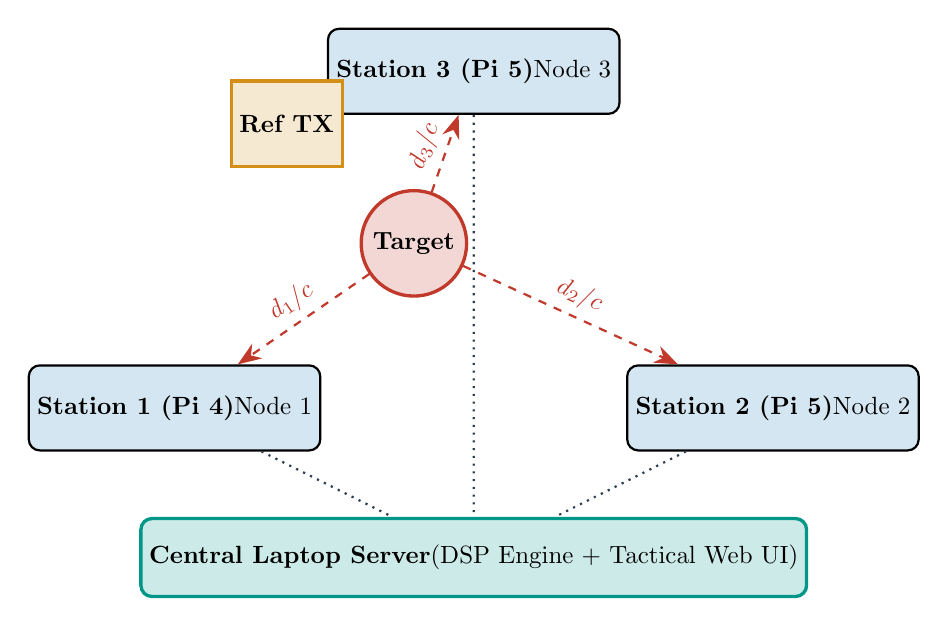
\begin{tikzpicture}[scale=0.95, every node/.style={scale=0.9}]
    % Ground Stations
    \node[draw, fill=secondaryblue!20, thick, rounded corners, minimum width=2.4cm, minimum height=1.2cm] (n1) at (0, 0) {\textbf{Station 1 (Pi 4)}\\Node 1};
    \node[draw, fill=secondaryblue!20, thick, rounded corners, minimum width=2.4cm, minimum height=1.2cm] (n2) at (8, 0) {\textbf{Station 2 (Pi 5)}\\Node 2};
    \node[draw, fill=secondaryblue!20, thick, rounded corners, minimum width=2.4cm, minimum height=1.2cm] (n3) at (4, 4.5) {\textbf{Station 3 (Pi 5)}\\Node 3};

    % Target Transmitter
    \node[draw=alertred, fill=alertred!20, very thick, circle, minimum size=1.4cm] (tgt) at (3.2, 2.2) {\textbf{Target}};

    % Reference Transmitter
    \node[draw=boxgold, fill=boxgold!20, very thick, rectangle, minimum size=1.2cm] (ref) at (1.5, 3.8) {\textbf{Ref TX}};

    % RF Waves from Target
    \draw[-{Stealth[length=3mm]}, thick, dashed, alertred] (tgt) -- node[above, sloped] {$d_1 / c$} (n1);
    \draw[-{Stealth[length=3mm]}, thick, dashed, alertred] (tgt) -- node[above, sloped] {$d_2 / c$} (n2);
    \draw[-{Stealth[length=3mm]}, thick, dashed, alertred] (tgt) -- node[above, sloped] {$d_3 / c$} (n3);

    % Central Laptop Server
    \node[draw=accentteal, fill=accentteal!20, very thick, rounded corners, minimum width=3.5cm, minimum height=1.1cm] (laptop) at (4, -2) {\textbf{Central Laptop Server}\\(DSP Engine + Tactical Web UI)};

    % Ethernet/WiFi links
    \draw[thick, dotted, darkslate] (n1) -- (laptop);
    \draw[thick, dotted, darkslate] (n2) -- (laptop);
    \draw[thick, dotted, darkslate] (n3) -- (laptop);
\end{tikzpicture}
\caption{The NanoSat TDOA Ground Architecture: Three remote ground receiver stations capture the target and reference signals simultaneously, streaming digital samples to the central server for processing.}
\end{figure}

% ============================================================================
\section{The Core Challenge: The Mystery of the Unsynchronized Clocks}
% ============================================================================

If radio waves travel at $300\text{ meters per microsecond}$ ($300\text{ m/}\mu\text{s}$), then:
\begin{itemize}
    \item $1\text{ microsecond error } (1\text{ }\mu\text{s}) \implies \mathbf{300\text{ meters error on the map}}!$
    \item $10\text{ nanoseconds error } (10\text{ ns}) \implies \mathbf{3.0\text{ meters error on the map}}!$
\end{itemize}

Commercial military TDOA systems solve this by plugging a $\$5{,}000$ Atomic Clock or GPS-Disciplined Oscillator (GPSDO) into every single receiver so that all stations take samples at the exact same picosecond. 

\textbf{Our Budget Constraint:} We are using $\$35$ RTL-SDR USB dongles and Raspberry Pis. They have NO atomic clocks. They have NO shared trigger wire. When Station 1 presses ``Record'', its operating system might begin recording 25 milliseconds after Station 2! 

\textbf{If their clocks are 25 milliseconds apart, that represents a $7{,}500\text{ kilometer}$ error!} How on earth do we fix this without expensive hardware?

\begin{conceptbox}{Our Secret Weapon: The Reference Transmitter (Pluto SDR)}
We place a stationary radio transmitter (ADALM-Pluto) at a known, surveyed ground location.
\begin{itemize}[leftmargin=*]
    \item The Reference Transmitter continuously broadcasts a known pseudo-random code alongside the target.
    \item Because we know \textit{exactly} where the Reference Transmitter is sitting, we can calculate with pencil and paper the exact physical travel time from the Reference to Station 1, Station 2, and Station 3.
    \item When Station 1 and Station 2 record, they record \textbf{both} the Target signal and the Reference signal in the exact same file!
    \item Any random startup delay or clock drift that affects Station 1 will affect \textit{both} the Reference and the Target identically.
    \item By subtracting the Reference delay from the Target delay, the unknown clock errors **vanish into thin air**!
\end{itemize}
\end{conceptbox}

% ============================================================================
\section{The Frequency Spectrum Plan: How Signals Share the Airwaves}
% ============================================================================

Our RTL-SDR receivers listen at a center frequency of \textbf{433.920 MHz} with a sampling rate of \textbf{2.4 MS/s} (Mega-samples per second). That gives us a listening window of $\pm 1.200\text{ MHz}$ around the center.

We place two distinct signals inside this single window:
\begin{enumerate}
    \item \textbf{Reference Transmitter (Pluto):} Broadcasts at \textbf{433.350 MHz} (Baseband: $-570\text{ kHz}$).
    \item \textbf{Target Transmitter (bladeRF):} Broadcasts at \textbf{434.490 MHz} (Baseband: $+570\text{ kHz}$).
\end{enumerate}

\begin{figure}[htbp]
\centering
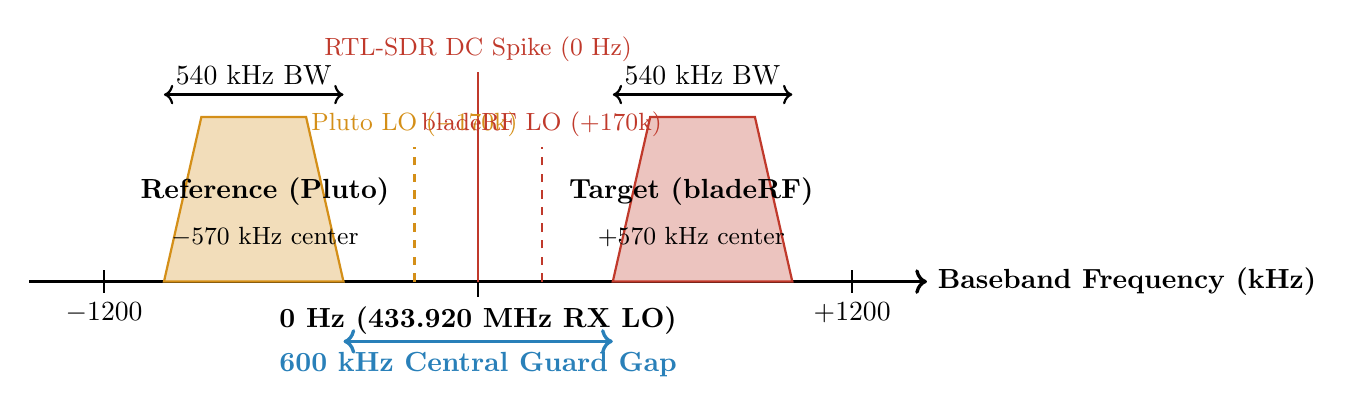
\begin{tikzpicture}[scale=0.95]
    % Frequency axis
    \draw[->, very thick] (-6, 0) -- (6, 0) node[right] {\textbf{Baseband Frequency (kHz)}};
    \draw[thick] (-5, 0.15) -- (-5, -0.15) node[below] {$-1200$};
    \draw[thick] (5, 0.15) -- (5, -0.15) node[below] {$+1200$};
    \draw[thick] (0, 0.2) -- (0, -0.2) node[below] {\textbf{0 Hz (433.920 MHz RX LO)}};

    % Reference Band (-570 kHz, width 540 kHz: [-840, -300])
    \fill[boxgold!30, draw=boxgold, thick] (-4.2, 0) -- (-3.7, 2.2) -- (-2.3, 2.2) -- (-1.8, 0) -- cycle;
    \node at (-2.85, 1.2) {\textbf{Reference (Pluto)}};
    \node at (-2.85, 0.6) {\small $-570\text{ kHz}$ center};
    \draw[<->, thick] (-4.2, 2.5) -- node[above] {$540\text{ kHz BW}$} (-1.8, 2.5);

    % Target Band (+570 kHz, width 540 kHz: [+300, +840])
    \fill[alertred!30, draw=alertred, thick] (1.8, 0) -- (2.3, 2.2) -- (3.7, 2.2) -- (4.2, 0) -- cycle;
    \node at (2.85, 1.2) {\textbf{Target (bladeRF)}};
    \node at (2.85, 0.6) {\small $+570\text{ kHz}$ center};
    \draw[<->, thick] (1.8, 2.5) -- node[above] {$540\text{ kHz BW}$} (4.2, 2.5);

    % Central Guard Gap
    \draw[<->, very thick, secondaryblue] (-1.8, -0.8) -- node[below] {\textbf{600 kHz Central Guard Gap}} (1.8, -0.8);

    % Spikes (DC & LO bleedthrough)
    \draw[thick, alertred] (0, 0) -- (0, 2.8) node[above] {\small RTL-SDR DC Spike ($0\text{ Hz}$)};
    \draw[thick, dashed, boxgold] (-0.85, 0) -- (-0.85, 1.8) node[above] {\small Pluto LO ($-170\text{k}$)};
    \draw[thick, dashed, alertred] (0.85, 0) -- (0.85, 1.8) node[above] {\small bladeRF LO ($+170\text{k}$)};
\end{tikzpicture}
\caption{The Authoritative Asymmetric Frequency Plan: The reference and target signals sit comfortably on opposite sides of the receiver center, leaving a pristine $600\text{ kHz}$ guard gap that traps all DC spikes and local oscillator (LO) leakage where digital filters can easily delete them.}
\end{figure}

\subsection{Why Is This Frequency Plan Brilliant?}
\begin{itemize}[leftmargin=*]
    \item \textbf{Total Separation:} Carrier difference $= 434.490 - 433.350 = \mathbf{1.140\text{ MHz}}$.
    \item \textbf{No Cross-Talk:} The inner edges sit at $-300\text{ kHz}$ and $+300\text{ kHz}$. Between them is a wide $600\text{ kHz}$ empty moat.
    \item \textbf{DC Spike Immunity:} Low-cost direct-conversion SDRs always generate an artificial voltage spike right at $0\text{ Hz}$ (center). In our design, $0\text{ Hz}$ falls directly into empty space, so it never pollutes the real signals!
\end{itemize}

% ============================================================================
\section{The Software Brain: Step-by-Step Algorithm Walkthrough}
% ============================================================================

When the stations finish their synchronous recording, the Central Server executes an automated 6-step signal processing pipeline in Python.

\begin{figure}[htbp]
\centering
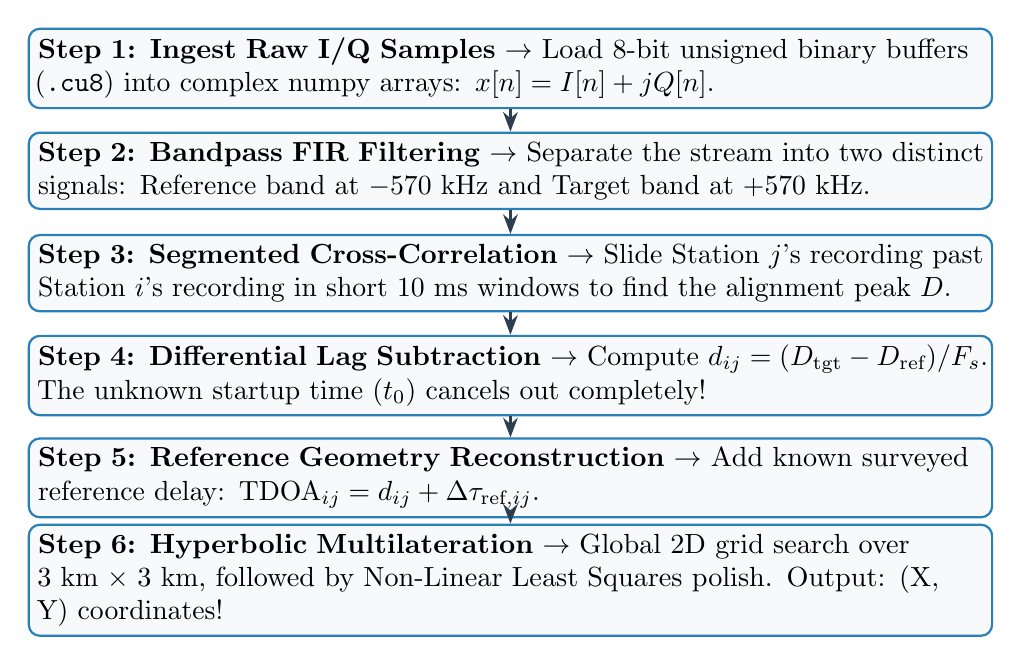
\begin{tikzpicture}[node distance=1.3cm, auto,
    block/.style={rectangle, draw=secondaryblue, fill=lightbg, thick, rounded corners, text width=12cm, minimum height=0.9cm, align=left},
    line/.style={draw, -{Stealth[length=2.5mm]}, thick, darkslate}]
    
    \node [block] (step1) {\textbf{Step 1: Ingest Raw I/Q Samples} $\rightarrow$ Load 8-bit unsigned binary buffers (\texttt{.cu8}) into complex numpy arrays: $x[n] = I[n] + jQ[n]$.};
    \node [block, below of=step1] (step2) {\textbf{Step 2: Bandpass FIR Filtering} $\rightarrow$ Separate the stream into two distinct signals: Reference band at $-570\text{ kHz}$ and Target band at $+570\text{ kHz}$.};
    \node [block, below of=step2] (step3) {\textbf{Step 3: Segmented Cross-Correlation} $\rightarrow$ Slide Station $j$'s recording past Station $i$'s recording in short $10\text{ ms}$ windows to find the alignment peak $D$.};
    \node [block, below of=step3] (step4) {\textbf{Step 4: Differential Lag Subtraction} $\rightarrow$ Compute $d_{ij} = (D_{\text{tgt}} - D_{\text{ref}}) / F_s$. The unknown startup time ($t_0$) cancels out completely!};
    \node [block, below of=step4] (step5) {\textbf{Step 5: Reference Geometry Reconstruction} $\rightarrow$ Add known surveyed reference delay: $\text{TDOA}_{ij} = d_{ij} + \Delta\tau_{\text{ref}, ij}$.};
    \node [block, below of=step5] (step6) {\textbf{Step 6: Hyperbolic Multilateration} $\rightarrow$ Global 2D grid search over $3\text{ km} \times 3\text{ km}$, followed by Non-Linear Least Squares polish. Output: (X, Y) coordinates!};

    \path [line] (step1) -- (step2);
    \path [line] (step2) -- (step3);
    \path [line] (step3) -- (step4);
    \path [line] (step4) -- (step5);
    \path [line] (step5) -- (step6);
\end{tikzpicture}
\caption{The Automated TDOA Digital Signal Processing (DSP) Pipeline.}
\end{figure}

\subsection{Deep-Dive: How Does Cross-Correlation Work?}
Cross-correlation is like sliding two identical comb teeth or puzzle pieces over each other:
$$R_{ba}[k] = \sum_{m} b[m + k] \cdot a^*[m]$$
\begin{itemize}[leftmargin=*]
    \item $a[m]$ is the signal chunk recorded by Station 1 (Base).
    \item $b[m]$ is the signal chunk recorded by Station 2 (Other).
    \item When we slide $b$ past $a$ by lag $k$, at the exact instant where the radio wave features match up, all mathematical samples multiply constructively and produce a giant sharp spike!
    \item The index of that spike tells us: \textbf{``Station 2 received this wavefront exactly $D$ samples later than Station 1.''}
\end{itemize}

\subsection{Sub-Sample Parabolic Interpolation}
At $2.4\text{ MS/s}$, each sample is $416.7\text{ ns}$ ($125\text{ meters}$). If we could only measure whole integer samples, our accuracy would be terrible ($\pm 125\text{ m}$).

To beat this limit, our algorithm looks at the highest correlation point and its two immediate neighbors ($y_{-1}, y_0, y_1$) and fits a smooth mathematical parabola through them:
$$\delta = \frac{1}{2} \cdot \frac{y_{-1} - y_{1}}{y_{-1} - 2y_0 + y_1}$$
This lets us pinpoint the peak to a tiny fraction of a sample (down to $0.01\text{ samples}$ or $< 2\text{ meters}$ under good SNR)!

% ============================================================================
\section{How Hyperbolas Pinpoint the Target on the Map}
% ============================================================================

When we measure that the target is $300\text{ meters}$ closer to Station 1 than Station 2, where could the target be?
\begin{itemize}
    \item It could be right between them.
    \item Or off to the north.
    \item Or off to the south.
\end{itemize}
The geometric shape of all points whose \textbf{difference in distance} to two fixed focal points is constant is called a \textbf{HYPERBOLA}.

\begin{figure}[htbp]
\centering
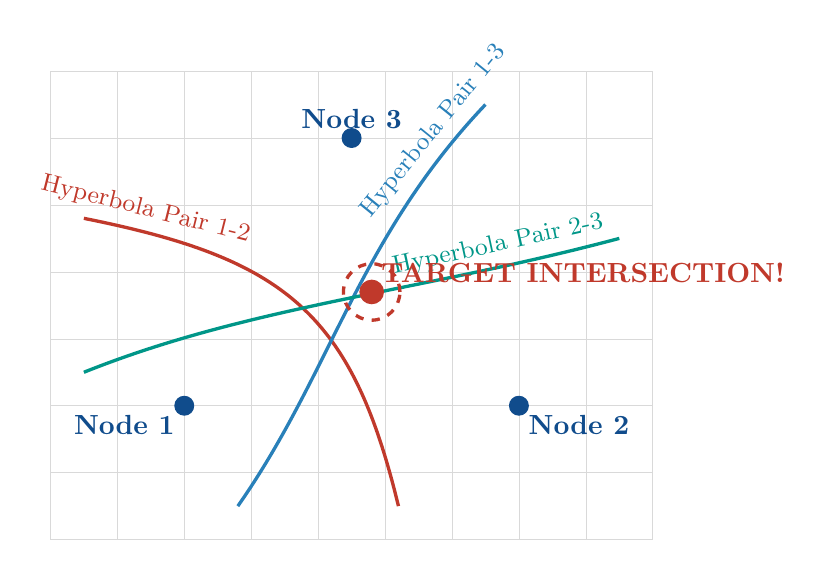
\begin{tikzpicture}[scale=0.85]
    % Axes
    \draw[help lines, color=gray!30] (-4, -3) grid (5, 4);

    % Ground Station Nodes
    \coordinate (N1) at (-2, -1);
    \coordinate (N2) at (3, -1);
    \coordinate (N3) at (0.5, 3);

    % Target Location
    \coordinate (TGT) at (0.8, 0.7);

    % Plot Nodes
    \filldraw[primaryblue] (N1) circle (4pt) node[below left] {\textbf{Node 1}};
    \filldraw[primaryblue] (N2) circle (4pt) node[below right] {\textbf{Node 2}};
    \filldraw[primaryblue] (N3) circle (4pt) node[above] {\textbf{Node 3}};

    % Hyperbolas (schematic curves)
    \draw[very thick, alertred] (-3.5, 1.8) .. controls (-0.5, 1.2) and (0.5, 0.4) .. (1.2, -2.5) 
        node[pos=0.1, above, sloped] {\small Hyperbola Pair 1-2};

    \draw[very thick, secondaryblue] (-1.2, -2.5) .. controls (0.2, -0.5) and (0.6, 1.5) .. (2.5, 3.5)
        node[pos=0.9, above, sloped] {\small Hyperbola Pair 1-3};

    \draw[very thick, accentteal] (-3.5, -0.5) .. controls (-1, 0.5) and (1.5, 0.7) .. (4.5, 1.5)
        node[pos=0.8, above, sloped] {\small Hyperbola Pair 2-3};

    % Target intersection
    \filldraw[alertred] (TGT) circle (5pt) node[above right] {\textbf{TARGET INTERSECTION!}};
    \draw[very thick, dashed, alertred] (TGT) circle (12pt);
\end{tikzpicture}
\caption{Hyperbolic Multilateration: Pair 1-2 gives the red curve. Pair 1-3 gives the blue curve. Pair 2-3 gives the green curve. All three curves intersect at exactly one unique point on Earth: the Target!}
\end{figure}

\subsection{Why 3 Stations Are the Golden Minimum}
\begin{itemize}[leftmargin=*]
    \item \textbf{1 Station:} Can only tell you a signal exists. Cannot tell distance or direction.
    \item \textbf{2 Stations:} Gives 1 time difference $\implies$ 1 continuous hyperbolic curve (infinite possible points).
    \item \textbf{3 Stations:} Gives 3 distinct pairs: $(1-2)$, $(1-3)$, and $(2-3)$. These generate 3 intersecting hyperbolas that cross at **one exact 2D coordinate $(X, Y)$**!
\end{itemize}

% ============================================================================
\section{The Web-Based Tactical Dashboard: Real-Time Radar}
% ============================================================================

Our central processing server runs a modern web-based Mission Control Dashboard built with HTML5, CSS3, JavaScript, and WebSockets.

\begin{figure}[htbp]
\centering
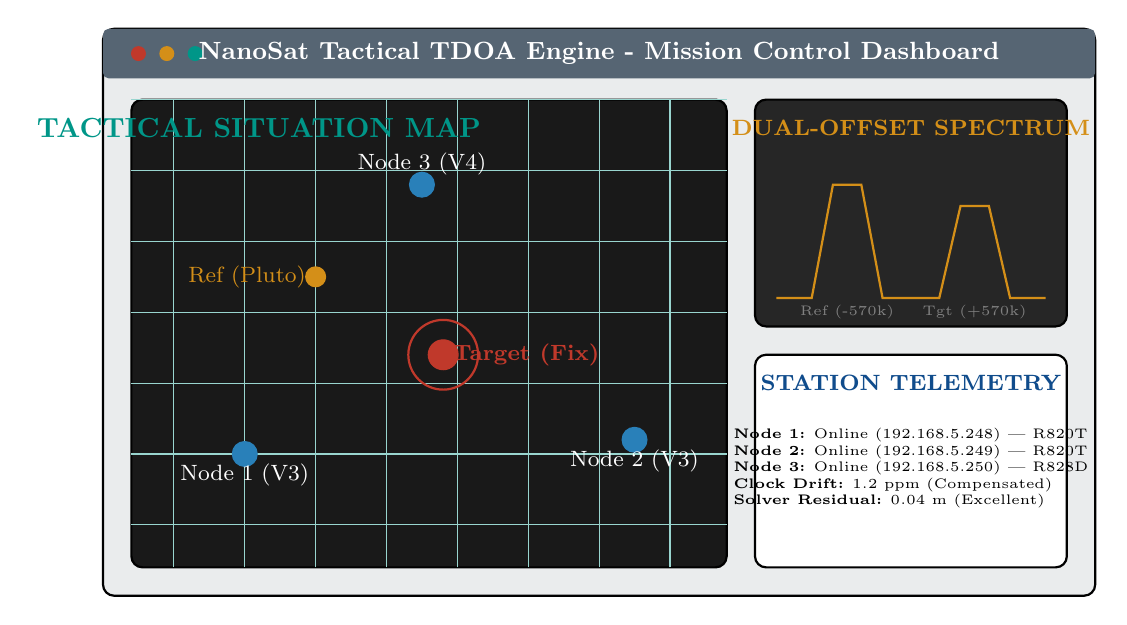
\begin{tikzpicture}[scale=0.9]
    % Browser Frame
    \draw[thick, fill=darkslate!10, rounded corners] (0, 0) rectangle (14, 8);
    \fill[darkslate!80, rounded corners=2pt] (0, 7.3) rectangle (14, 8);
    \fill[alertred] (0.5, 7.65) circle (3pt);
    \fill[boxgold] (0.9, 7.65) circle (3pt);
    \fill[accentteal] (1.3, 7.65) circle (3pt);
    \node[white, font=\bfseries\small] at (7, 7.65) {NanoSat Tactical TDOA Engine - Mission Control Dashboard};

    % Left Panel: Tactical Map
    \draw[thick, fill=black!90, rounded corners] (0.4, 0.4) rectangle (8.8, 7.0);
    \draw[accentteal!40, step=1.0] (0.4, 0.4) grid (8.8, 7.0);
    \node[accentteal, font=\bfseries] at (2.2, 6.6) {TACTICAL SITUATION MAP};
    % Nodes on map
    \filldraw[secondaryblue] (2.0, 2.0) circle (5pt) node[below, text=white, font=\footnotesize] {Node 1 (V3)};
    \filldraw[secondaryblue] (7.5, 2.2) circle (5pt) node[below, text=white, font=\footnotesize] {Node 2 (V3)};
    \filldraw[secondaryblue] (4.5, 5.8) circle (5pt) node[above, text=white, font=\footnotesize] {Node 3 (V4)};
    \filldraw[boxgold] (3.0, 4.5) circle (4pt) node[left, text=boxgold, font=\footnotesize] {Ref (Pluto)};
    \filldraw[alertred] (4.8, 3.4) circle (6pt) node[right, text=alertred, font=\bfseries\footnotesize] {Target (Fix)};
    \draw[alertred, thick] (4.8, 3.4) circle (14pt);

    % Right Top: Live RF Spectrum
    \draw[thick, fill=black!85, rounded corners] (9.2, 3.8) rectangle (13.6, 7.0);
    \node[boxgold, font=\bfseries\footnotesize] at (11.4, 6.6) {DUAL-OFFSET SPECTRUM};
    \draw[boxgold, thick] (9.5, 4.2) -- (10.0, 4.2) -- (10.3, 5.8) -- (10.7, 5.8) -- (11.0, 4.2) -- (11.8, 4.2) -- (12.1, 5.5) -- (12.5, 5.5) -- (12.8, 4.2) -- (13.3, 4.2);
    \node[font=\tiny, text=gray] at (10.5, 4.0) {Ref (-570k)};
    \node[font=\tiny, text=gray] at (12.3, 4.0) {Tgt (+570k)};

    % Right Bottom: Station Health & Telemetry
    \draw[thick, fill=white, rounded corners] (9.2, 0.4) rectangle (13.6, 3.4);
    \node[primaryblue, font=\bfseries\footnotesize] at (11.4, 3.0) {STATION TELEMETRY};
    \node[font=\tiny, align=left] at (11.4, 1.8) {
        \textbf{Node 1:} Online (192.168.5.248) | R820T\\
        \textbf{Node 2:} Online (192.168.5.249) | R820T\\
        \textbf{Node 3:} Online (192.168.5.250) | R828D\\
        \textbf{Clock Drift:} $1.2\text{ ppm}$ (Compensated)\\
        \textbf{Solver Residual:} $0.04\text{ m}$ (Excellent)
    };
\end{tikzpicture}
\caption{Mockup of the Tactical Web Dashboard: Live hyperbolic map display, dual-offset spectral FFT waterfall, and ground station telemetry indicators.}
\end{figure}

\subsection{Key Features of the Web Interface}
\begin{enumerate}[leftmargin=*]
    \item \textbf{Leaflet GPS Map:} Overlays the true ground coordinates of your campus or field test site with satellite imagery.
    \item \textbf{Hyperbolic Isochrone Contours:} Dynamically plots the colorful curved hyperbolic lines on the map so you can visually see them intersect at the target.
    \item \textbf{Live FFT Spectrum Display:} Shows the raw $2.4\text{ MS/s}$ baseband spectrum, displaying the Pluto peak at $-570\text{ kHz}$ and the bladeRF peak at $+570\text{ kHz}$.
    \item \textbf{Station Health Watchdog:} Automatically monitors each Raspberry Pi's CPU temperature, free SD card space, and USB stream stability.
\end{enumerate}

% ============================================================================
\section{Step-by-Step Lab Action Plan for Tomorrow}
% ============================================================================

\begin{safetybox}{CRITICAL RF SAFETY RULES (Read Before Touching Anything!)}
\begin{enumerate}[leftmargin=*]
    \item \textbf{NO Over-the-Air Transmission:} Transmitting on $433\text{ MHz}$ without official frequency clearance in Pakistan is illegal. Tomorrow's lab session is strictly \textbf{RECEIVE-ONLY} and \textbf{CLOSED-COAXIAL}.
    \item \textbf{NEVER Connect TX Directly to RTL-SDR:} Transmitters like bladeRF put out up to $+10\text{ dBm}$ ($10\text{ mW}$). An RTL-SDR receiver LNA begins burning out above $+10\text{ dBm}$ and compresses at $-20\text{ dBm}$. Connecting them directly will permanently destroy the RTL-SDR dongle!
    \item \textbf{Supervisor Approval First:} Do NOT turn on any RF transmitter until Sir Ahsan or the lab engineer has inspected the attenuators and signed off on the power budget.
\end{enumerate}
\end{safetybox}

\subsection{Phase 1: Receive-Only Hardware Verification}
Tomorrow morning in the lab, follow this sequence:

\begin{enumerate}[leftmargin=*]
    \item \textbf{Check Dongles on USB 3.0 Ports:}
    Plug the RTL-SDRs into the \textbf{Blue USB 3.0 ports} of each Raspberry Pi. (USB 2.0 can drop samples at high speeds).
    
    \item \textbf{Run the Hardware Identifier Command:}
    On each Pi terminal, type:
    \begin{lstlisting}[language=bash, basicstyle=\small\ttfamily, backgroundcolor=\color{lightbg}, frame=single]
rtl_test -t
    \end{lstlisting}
    \begin{itemize}
        \item \textbf{Station 1 \& 2 (V3):} Terminal must say: \texttt{Found Rafael Micro R820T tuner}.
        \item \textbf{Station 3 (V4):} Terminal must say: \texttt{Found Rafael Micro R828D tuner}. If it says ``error'' or fails, run \texttt{setup\_pi.sh} to compile the V4 blog driver!
    \end{itemize}

    \item \textbf{60-Second USB Streaming Test:}
    Test if the Pi can stream $2.4\text{ MS/s}$ continuously without dropping data:
    \begin{lstlisting}[language=bash, basicstyle=\small\ttfamily, backgroundcolor=\color{lightbg}, frame=single]
rtl_sdr -f 433920000 -s 2400000 -n 144000000 /tmp/test_rx.cu8
    \end{lstlisting}
    \begin{itemize}
        \item Look at the screen: there should be \textbf{zero dropped bytes} (no \texttt{ll+} or \texttt{cb} errors).
        \item Verify file size: Type \texttt{ls -l /tmp/test_rx.cu8}. It must be \textbf{exactly 288,000,000 bytes} ($288\text{ MB}$)!
        \item Clean up: \texttt{rm /tmp/test_rx.cu8}.
    \end{itemize}
\end{enumerate}

\subsection{Phase 2: Inspecting the Lab RF Rig (With Sir Ahsan)}
Before any transmitters are enabled, inspect the bench components:
\begin{itemize}[leftmargin=*]
    \item \textbf{2-Way Combiner:} Check model number (must have $>20\text{ dB}$ port isolation so Pluto and bladeRF don't leak power into each other).
    \item \textbf{30 dB Attenuator:} Check frequency rating (must cover up to $500\text{ MHz}$) and power rating ($> 2\text{ Watts}$).
    \item \textbf{3-Way Splitter:} Check that all 3 coaxial output cables are \textbf{identical in length} (within $1\text{ cm}$).
    \item \textbf{Spectrum Analyzer Verification:} Connect the splitter output to the lab's Spectrum Analyzer / Power Meter. Verify that the combined signal power is strictly \textbf{below $-30\text{ dBm}$}.
\end{itemize}

% ============================================================================
\section{Viva \& Examiner Cheat Sheet: How to Answer Sir Ahsan}
% ============================================================================

When your supervisor or examiner asks you tough questions, use these clear, professional answers:

\vspace{0.2cm}
\noindent\textbf{Q1: ``How can you do TDOA with cheap RTL-SDRs when their clocks are completely unsynchronized?''}\\
\textit{\textbf{Answer:}} ``We use an Asymmetric Dual-Offset Reference-Assisted architecture. We place a stationary reference transmitter at a known surveyed position. Because both reference and target signals are recorded simultaneously in the same baseband buffer, subtracting the measured reference lag from the target lag completely cancels the receiver's unknown startup time offset ($t_0$) and receiver LO drift.''

\vspace{0.2cm}
\noindent\textbf{Q2: ``What about sample clock drift between different dongles? Doesn't that ruin the correlation?''}\\
\textit{\textbf{Answer:}} ``Yes! Over 1 second, a $4\text{ ppm}$ differential drift shifts the signal by $9.6\text{ samples}$ ($1{,}200\text{ meters}$), which would destroy correlation. We solve this by segmenting the processing into short $10\text{ ms}$ windows where the drift is only $0.096\text{ samples}$ ($12\text{ meters}$), tracking the drift dynamically segment-by-segment and averaging with a median filter.''

\vspace{0.2cm}
\noindent\textbf{Q3: ``Why did you choose 433.350 MHz and 434.490 MHz?''}\\
\textit{\textbf{Answer:}} ``They are symmetrically offset by $\pm 570\text{ kHz}$ from the receiver's center frequency ($433.920\text{ MHz}$). This creates a $600\text{ kHz}$ central guard gap that isolates both signals from zero-IF receiver DC spike noise and transmitter LO carrier bleedthrough.''

\vspace{0.2cm}
\noindent\textbf{Q4: ``How do you solve the position from the time delays?''}\\
\textit{\textbf{Answer:}} ``We use a two-stage solver. Stage 1 executes an exhaustive 2D grid search over a $3\text{ km} \times 3\text{ km}$ area to find the global minimum, guaranteeing we never get stuck in local minima. Stage 2 executes a Levenberg-Marquardt non-linear least squares polish starting from that point to reach sub-meter numerical precision.''

\vspace{0.2cm}
\noindent\textbf{Q5: ``What is the difference between your synthetic test results and physical lab results?''}\\
\textit{\textbf{Answer:}} ``Our synthetic tests prove that the mathematics, coordinate geometry, sign conventions, and algorithm code are 100\% consistent and bug-free. However, physical real-world accuracy will be determined by RF signal-to-noise ratio, multi-path reflections from campus buildings, and analog filter group delay variations between V3 and V4 dongles, which we are measuring in the lab.''

\end{document}
